\documentclass{article}

% Language setting
% Replace `english' with e.g. `spanish' to change the document language
\usepackage[utf8]{inputenc}
\usepackage[russian]{babel}

% Set page size and margins
% Replace `letterpaper' with `a4paper' for UK/EU standard size
\usepackage[a4paper,top=2cm,bottom=2cm,left=3cm,right=3cm,marginparwidth=1.75cm]{geometry}

% Useful packages
\usepackage{amsmath}
\usepackage{graphicx}
\usepackage[colorlinks=true, allcolors=blue]{hyperref}
\usepackage{listings}
\usepackage{float   }

\lstdefinestyle{C}{               
    numbers=left,
    numbersep=10pt,
    breaklines=true
}

\title{Дерево ван Эмде Боаса}
\author{Голобородько Димитрий}

\begin{document}
\maketitle


\section{Введение}
\subsection{Суть и назначение}
Дерево ван Эмде Боаса — поисковая структура данных, представляющая собой дерево поиска, позволяющее хранить уникальные целые неотрицательные числа в интервале $[0;2^k)$ и осуществлять над ними основные операции поисковой структуры данных за $O(log{k})$ при затратах памяти $\Theta(2^k)$.
\subsection{История}
Структура разработана осенью 1974 года Питером ван Эмде Боасом во время его трёхмесячного пост-докторского резиденства в Корнеллском университете и представлена в 1975 году. Автор структуры отмечает, что на его ранние публикации оказывал влияние культурный климат в алгоритмике середины 1970-х годов, на фоне которого структура была разработана для машины указателей (pointer machine). Причина в том, что рекурсивный подход требует адресных вычислений. Данные операции не допускались в модели машины с произвольным доступом (RAM), которая была стандартной моделью в развивающейся области исследований проектирования и анализа алгоритмов в 1974 году. Недостатком этого подхода является то, что он приводит к довольно сложным алгоритмам, которые и сегодня трудно корректно реализовать. 
\subsection{Применение}
Данное дерево может применяться в задачах, где требуется поисковая структура данных для множества уникальных целых неотрицаетльных чисел, верхняя граница которого известна заранее, либо ограничена типом данных, при этом количество чисел достаточно велико, чтобы оправдать накладные расходы памяти.
В сети встречаются упоминания применения дерева ван Эмде Боаса в алгоритмах на графах и вычислительной геометрии, а также в сетевых маршрутизаторах.
\section{Описание}
\subsection{Поддерживаемые операции}
\begin{itemize}
    \item member - проверка наличия числа в структуре
    \item insert - вставка числа
    \item remove - удаление числа
    \item successor - поиск следующего по возрастанию числа за данным
    \item predecessor - поиск следующего по убыванию числа за данным
    \item min, max - посик минимального, максимального хранимых чисел 
\end{itemize}
\subsection{Вспомогательные функции}
Для поддержки тех размерностей поддеревьев, из значений которых целый квадратный корень не извлекается, введены следующие вспомогательные функции:
\begin{itemize}
    \item lower\_sqrt(x) - ''нижний квадратный корень'', равен $2^{\lfloor\log_{2}(x)/2\rfloor}$
    \item upper\_sqrt(x) - ''верхний квадратный корень'', равен $2^{\lceil\log_{2}(x)/2\rceil}$
\end{itemize}
При этом $x = upper\_sqrt(x) * lower\_sqrt(x)$, а когда $\sqrt{x}$ - целое, верно $\sqrt{x} = upper\_sqrt(x) = lower\_sqrt(x)$
\begin{itemize}
    \item low(u, x) - младшие $2^{\lfloor\log_{2}(u)/2\rfloor}$ бит номера элемента x, вычисляются как $\lfloor{x/lower\_sqrt(u)}\rfloor$ где u - размерность текущего поддерева
    \item high(u, x) - старшие $2^{\lceil\log_{2}(u)/2\rceil}$ бит номера x, вычисляются как $x\mod{lower\_sqrt()}$  где u - размерность текущего поддерева
    \item index(u, x, y) - совмещает номер элемента из старших бит x и младших бит y, вычисляется как $x*lower\_sqrt(u) + y$, где u - размерность текущего поддерева
    
\end{itemize}
\subsection{Структура данных}
Дерево ван Эмде Боаса является рекурсивной структурой, каждый узел которого является корнем поддерева и содержит в себе:
\begin{itemize}
    \item u - размерность поддерева, элементов
    \item min, max - хранят минимальный и максимальный элемент поддерева
    \item summary - указатель на справочную структуру, которая также является деревом ван Эмде Боаса с размерностью $upper\_sqrt(u)$ элементов 
    \item cluster - массив из $upper\_sqrt(u)$ указателей на поддеревья с размерностью $upper\_sqrt(u)$
\end{itemize}

\begin{figure}[H]
    \centering
    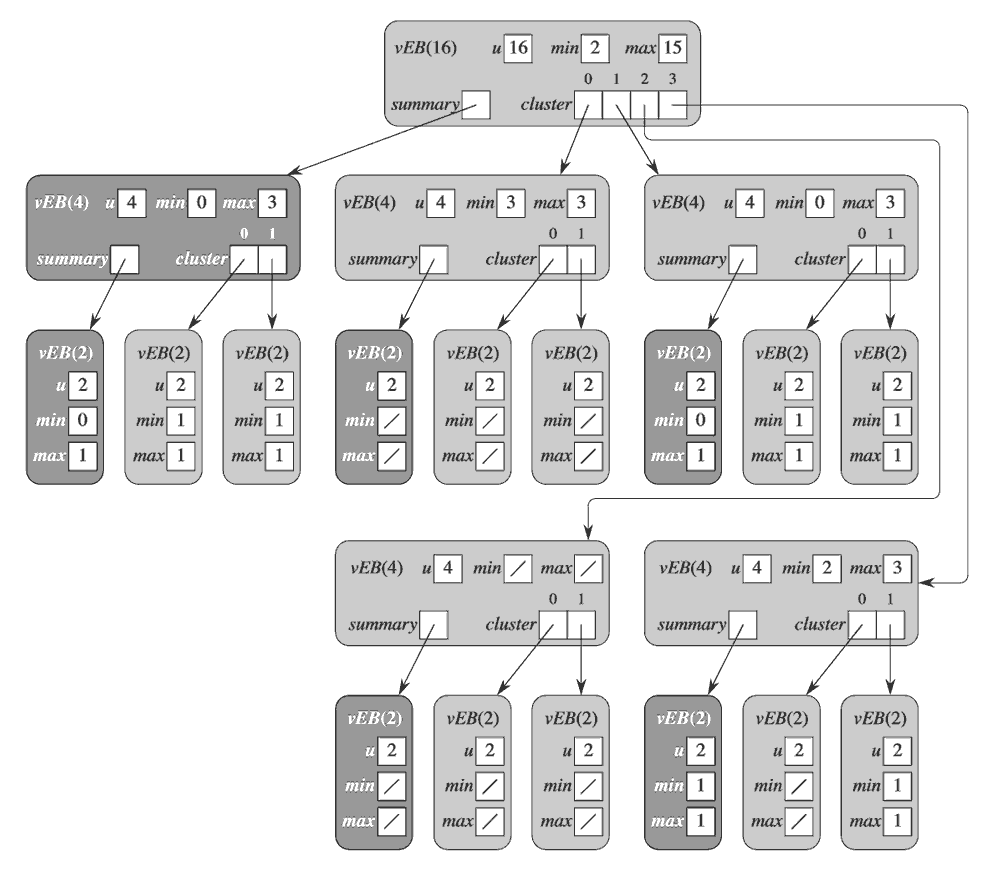
\includegraphics[width=0.9\textwidth]{veb.png}
    \caption{Дерево ван Эмде Боаса размерностью 16, содержащее числа \{2, 3, 4, 5, 7, 14, 15\}}
\end{figure}

\subsection{Входные данные и ограничения}
Оргинальная структура, представленная Питером ван Эмде Боасом требует корректности входных данных, а именно, не гарантирует корректного удаления не существующего элемента, добавления уже существующего элемента. Размерность дерева u должна быть степенью числа 2. Все операции на дереве размерностью u подразумевают работу только с числами из интервала $[0;u)$.
\section{Формальная постановка задачи}
Исследовать и реализовать дерево ван Эмде Боаса в виде набора функций для создания и удаления рекурсивной структуры дерева, исполнения набора поддерживаемых операций (member, insert, remove, successor, predecessor, min, max).
\section{Реализация}
В реализации в рамках данного доклада для значения элемента выбран тип unsigned int, что ограничивает максимальную размерность дерева значением в $2^{32}-1$ элементов, при этом последний элемент unsigned int ($2^{32}-1$) зарезервирован как флаг, обозначающий пустой элемент NIL в полях min и max.
\subsection{Структура узла}
\begin{lstlisting}[language=C,style=C]
typedef struct veb_node veb;
struct veb_node
{
    unsigned int u;
    unsigned int min;
    unsigned int max;
    veb *summary;
    veb **cluster;
};
\end{lstlisting}
\subsection{Реализация вспомогательных функций}
\begin{lstlisting}[language=C,style=C]
const unsigned int NIL = -1;

unsigned int veb_upper_sqrt(unsigned int u) {
    return pow(2, ceil(log2(u)/2));
}

unsigned int veb_lower_sqrt(unsigned int u) {
    return pow(2, floor(log2(u)/2));
}

unsigned int veb_high(unsigned int u,  unsigned int x) {
    return floor(x/veb_lower_sqrt(u));
}

unsigned int veb_low(unsigned int u, unsigned int x) {
    return x % veb_lower_sqrt(u);
}

unsigned int veb_index(unsigned int u, unsigned int x, unsigned int y) {
    return x*veb_lower_sqrt(u)+y;
}
\end{lstlisting}
\subsection{Min, max}
Значения минимума и максимума дерева ван Эмде Боаса, хрянятся в полях структуры корня, поэтому могут быть получены за константное время.
\begin{lstlisting}[language=C,style=C]
unsigned int veb_tree_minimum(veb* v) {
    return v->min;
}
unsigned int veb_tree_maximum(veb* v) {
    return v->max;
}
\end{lstlisting}
\subsection{Member}
\begin{lstlisting}[language=C,style=C]
unsigned int veb_tree_member(veb* v, unsigned int x){
    return
        x == v->min || x == v->max ? 1 :
        v->u == 2 ? 0 :
        veb_tree_member(v->cluster[veb_high(v->u,x)], veb_low(v->u, x));
}
\end{lstlisting}
Строка 3 проверяет случай, в котором искомый элемент x является максимальным или минимальным в дереве, и возвращает истину, если это так. Строка 4 проверяет случай, в котором поддерево размерностью $u=2$ не имеет элементов, возвращает ложь если это так. В противном случае происходит рекурсивное углубление в поддерево с индексом high(u, x) и поиск числа $x = low(u, x)$
\subsection{Successor, predecessor}
\begin{lstlisting}[language=C,style=C]
unsigned int veb_tree_successor(veb* v, unsigned int x){
    if (v->u == 2) {
        if (x == 0 && v->max == 1) {
            return 1;
        } else {
            return NIL;
        }
    } else if (v->min != NIL && x < v->min)
    {
        return v->min;
    } else {
        unsigned int max_low = veb_tree_maximum(v->cluster[veb_high(v->u,x)]);
        if (max_low != NIL && veb_low(v->u, x) < max_low) {
            unsigned int offset = veb_tree_successor(v->cluster[veb_high(v->u, x)], veb_low(v->u,x));
            return veb_index(v->u, veb_high(v->u, x), offset);
        }
        else {
            unsigned int succ_cluster = veb_tree_successor(v->summary, veb_high(v->u,x));
            if (succ_cluster == NIL)
            {
                return NIL;
            } else {
                unsigned int offset = veb_tree_minimum(v->cluster[succ_cluster]);
                return veb_index(v->u, succ_cluster, offset);
            }
        }
    }
}
\end{lstlisting}
\begin{lstlisting}[language=C,style=C]
unsigned int veb_tree_predecessor(veb* v, unsigned int x){
    if (v->u == 2) {
        if (x == 1 && v->min == 0) {
            return 0;
        } else {
            return NIL;
        }
    } else if (v->max != NIL && x > v->max)
    {
        return v->max;
    } else {
        unsigned int min_low = veb_tree_minimum(v->cluster[veb_high(v->u, x)]);
        if (min_low != NIL && veb_low(v->u, x) > min_low) {
            unsigned int offset = veb_tree_predecessor(v->cluster[veb_high(v->u, x)], veb_low(v->u, x));
            return veb_index(v->u, veb_high(v->u, x), offset);
        } else {
            unsigned int pred_cluster = veb_tree_predecessor(v->summary, veb_high(v->u, x));
            if (pred_cluster == NIL) {
                if (v->min != NIL && x > v->min){
                    return v->min;
                } else {
                    return NIL;
                }
            } else {
                unsigned int offset = veb_tree_maximum(v->cluster[pred_cluster]);
                return veb_index(v->u, pred_cluster, offset);
            }
        }
    }
}
\end{lstlisting}
Строки 2-7 проверяют базовый случай 



\section{Список литературы}
\begin{itemize}
    \item \url{https://edutechlearners.com/download/Introduction_to_algorithms-3rd\%20Edition.pdf}
    \item \url{https://www.mi.fu-berlin.de/inf/groups/ag-ti/theses/download/Ehrhardt15.pdf}
    \item \url{https://mathoverflow.net/questions/2245/determining-the-space-complexity-of-van-emde-boas-trees}
    \item \url{https://web.stanford.edu/class/archive/cs/cs166/cs166.1166/lectures/14/Slides14.pdf}
    \item \url{https://toc.csail.mit.edu/node/757}
    \item \url{https://fileadmin.cs.lth.se/cs/Personal/Rolf_Karlsson/lect12.pdf}
    \item \url{https://leprofesseur.org/algorithms-lecture-019-van-emde-boas-veb-trees/}
\end{itemize}


\end{document}